L'objectif de ce travail est de fournir une base pour celui qui doit écrire un rapport pour le cours de Mr Jaumain. Il commence par une suite d'exemples suffisante pour pouvoir établir un premier rapport correct. Ensuite, une série d'autres exemples montre comment améliorer sa présentation pour l'étudiant qui le souhaite. Ce rapport, comme celui de l'étudiant doit comporter un titre, une table des matières, un résumé de l'objectif poursuivi, le texte découpé en chapitre, une conclusion, les références et le contenu du répertoire associé.  
\section {Une première approche très simple}
Vous découpez votre travail en chapitre (section), en sous-chapitre (subsection) et en sous-sous-chapitre (subsubsection)
\subsection {Un chapitre simple}
Il suffit de taper le texte au kilomètre. \emph{Il est possible d'insister} sur un passage.
\subsection {Vérification de l'orthographe}
Vous appelez la commande :
\lstset{frame=trBL}
\begin{lstlisting}
aspell -t - -encoding='iso8859-15' -c VotreFichier.tex
\end{lstlisting}
\subsection {Une énumération}
Si vous devez utiliser des puces :
\begin{itemize}
\item point 1
\item point 2
\end{itemize}
Si vous devez énumérer :
\begin{enumerate}
\item point 1
\item point 2
\end{enumerate}
Vous pouvez mélanger à autant de niveau que vous le souhaitez.
\subsection{Un tableau}
\begin{tabular}{|l|l||c||r|} %left ou r ou c ou p[dimension]
\hline
Jour & Heures & Local & Cours \\
\hline
Mardi    &  3..4  & 503 & Système\\
Mardi    &  5..8  & 503 & Sécurité\\
\hline
Mercredi  &  1..2  &  201 & Assembleur\\
Mercredi  &  3..4  &  003 & Labo assembleur\\
\hline
\end{tabular}
\subsection {Intégrer une source}
Pour énumérer une source, vous pouvez préciser ce que vous souhaitez avec lstset. 
\lstset{language=c,frame=trBL}
\begin{lstlisting}
MOV EAX,10 ; place 10 dans le registre EAX
ADD EAX,20 ; ajoute 20 au contenu de EAX
\end{lstlisting}
\subsection {Intégrer un graphique}
Vous pouvez intégrer un graphique mais il faut qu'il soit en format eps.\\
Vous pouvez dessiner avec l'outil oodraw qui permet d'exporter votre dessin dans ce format eps.\\
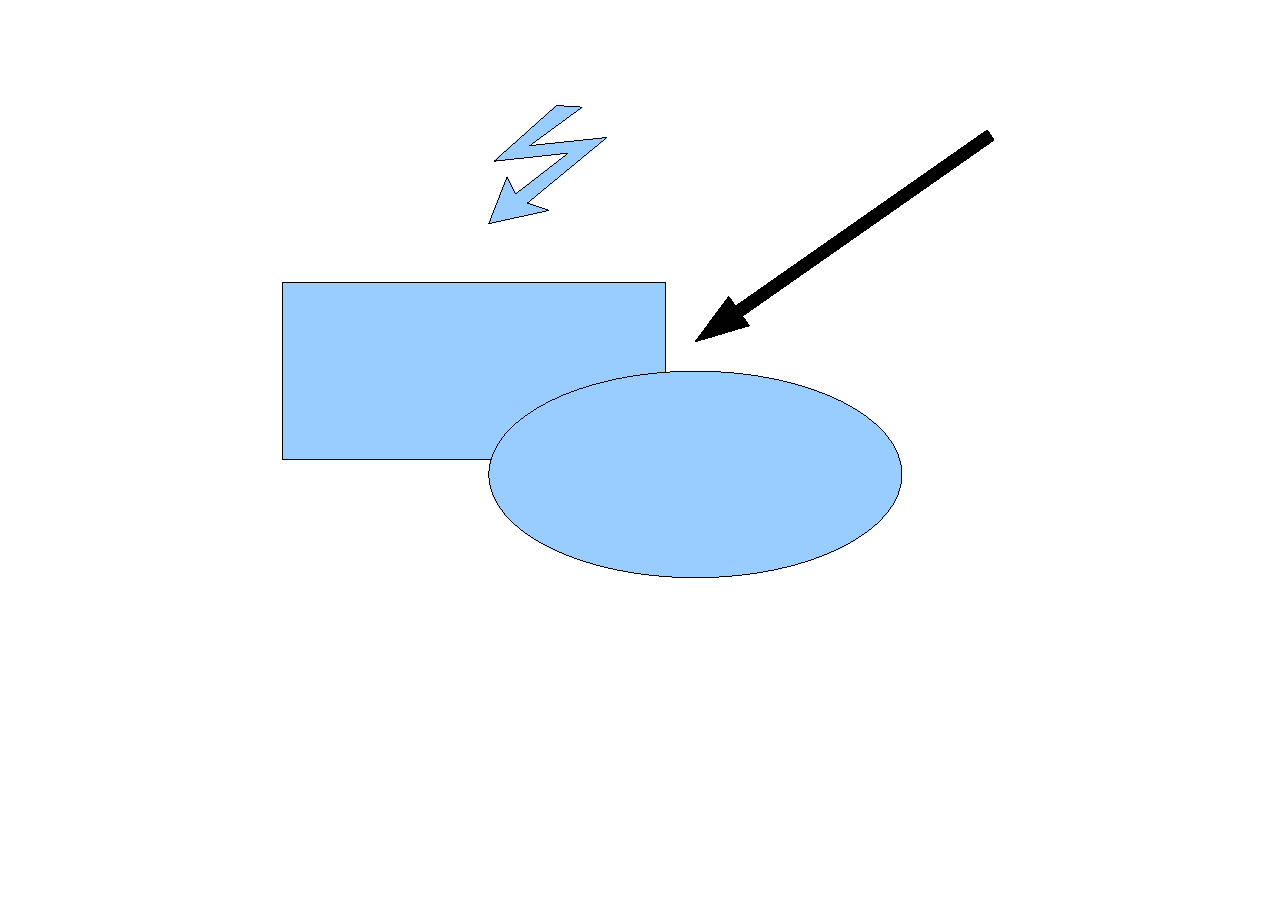
\includegraphics[width=10cm]{Dessin.eps}
\subsection {Mode mathématique}
C'est un des points forts de latex qui permet d'écrire des formules mais aussi des caractères spéciaux tels que :
$2^{32} \approx 10^{9}$ car $\log{_{10}}{2} \approx 0.3$ et $32*0.3 \approx 9$.
\subsection {Quelques trucs faciles}
\begin{itemize}
\item \verb+\\+ permet de passer à la ligne suivante.
\item \verb+\\[2cm]+ permet de passer à la ligne suivante + une tabulation verticale de 2cm. Sont autorisés mm, cm et pts.
\item \verb+\newpage+ permet de forcer un passage à la page suivante.
\end{itemize}
\subsection {Compiler le texte}
Un script permet d'automatiser cette compilation:
\begin{lstlisting}
#! /bin/sh
FN=Mrapport # Le nom du document.
latex $FN.tex
latex $FN.tex # 2 passages pour la TOC
rm $FN.aux $FN.log $FN.out
dvips $FN.dvi -o $FN.ps
rm $FN.dvi
gv $FN.ps # pour visualiser et imprimer
\end{lstlisting}

\section{Pour aller un peu plus loin...}
\subsection{Configuration de lstlisting}
% Le manuel se trouve dans le howto.
\lstset{language=C,% Assembleur, TeX, tcl, basic, cobol, fortran, logo, make, pascal, perl, prolog, {}
   	commentstyle=\scriptsize\ttfamily\slshape, % style des commentaires
	basicstyle=\scriptsize\ttfamily, % style par défaut
   	keywordstyle=\scriptsize\rmfamily\bfseries,% style des mots-clés
   	backgroundcolor=\color[rgb]{.9,.9,.9}, % couleur de fond : gris clair
   	framerule=0.5pt,% Taille des bords
   	frame=trbl,% Style du cadre
 	frameround=tttt, % Bords arrondis 
   	tabsize=1, % Taille des tabulations
 	extendedchars=true, % 
 	showspaces=false, % Ne montre pas les espaces 
 	showstringspaces=false, % Ne montre pas les espaces entre ''
 	numbers=left, % Numérote les lignes à gauche
 	numberstyle=\tiny, % La numérotation se fait en petit
 	xrightmargin=-1cm, % Retrait gauche 
 	xleftmargin=-1cm, % Retrait droit
   	escapechar=@}  % Caractère d'échappement, permet des commandes latex dans la source

\begin{lstlisting}
main() {
	int i;  // Pour récupérer le nombre de caractères écrits
	tab[10] Buffer='Hello'; // Le buffer
	i=write(1,Buffer,5); // La @$\frac{1}{2}$@ du buffer
	exit(0);
}
\end{lstlisting}

\subsection{Configuration des énumérations}
Vous pouvez remplacer le tiret d'une liste à puce par un caractère
\begin{list}{]}{}
\item Point 1
\item Point 2
	\begin{list}{$\bullet$}{}
	\item Point 2.1
	\item Point 2.2
	\item Point 2.3
	\end{list}
\item Point 3
\end{list}

\subsection{Mémoriser son style}
todo macro Azza

\subsection{Mémoriser une nouvelle commande}
todo mon travail latex

\subsection{Construire un tableau complexe}
todo  Voir Azza

\subsection{Mémoriser un nouvel environnement}
todo Voir Azza

\subsection{Mémoriser une font}
todo Voir mon travail latex

\subsection{Environnement figure}
todo voir Azza

\subsection{Environnement minipage}
todo voir Azza

\subsection{Mathématiques}
% use package amsmath, amsfont, amssymb peuvent être utiles.

Quelques exemples des possibilités mathématiques :

La fonction $e^x$ est strictement croissante sur $R$ et $\forall x \in R$.

\begin{equation}
\frac{\partial}{\partial y}\int_E f(x,y)\,dx = \int_E \frac{\partial f(x,y)}{\partial y}\,dx
\end{equation}

$$\lim_{x \to +\infty} \frac{\ln x}{x} = 0$$

$$ 10 \textrm{ dixièmes} = 1 $$

\begin{equation}
\sum_{k=1}^n k = \frac{n(n+1)}{2}
\end{equation}

\begin{equation}
\int_0^{+\infty} x^n e^{-x}\,dx = n!
\end{equation}

$$\left \{\begin{array}{c}x+y=1\\x-y=1\end{array}\right.$$

\begin{equation}
\left( \begin{array}{cc} a & b \\ c & d \end{array} \right) \cdot
\left( \begin{array}{cc} 0 & 1 \\ 0 & 0 \end{array} \right) =
\left( \begin{array}{cc} 0 & a \\ 0 & c \end{array} \right)
\end{equation}

$$\widehat{ab} + \widehat{bc} + \widehat{cb} = 180$$

$$\overrightarrow{ab} + \overrightarrow{ac} = \overrightarrow{ad}$$



\section{Conclusions}
Ce travail montre, qu'en quelques minutes, on peut déjà fournir un travail présenté de façon professionnelle, lisible par tous et dans un format standard.
Pour l'étudiant qui ne souhaite pas consacrer du temps à affiner sa présentation, le chapitre 2 n'est pas utile.
Pour ne pas avoir de soucis, les commandes à utiliser pour obtenir un document postcript sont latex et dvips, il ne faut jamais utiliser pdflatex. 

Ce document peut être encore complété avec d'autres exemples qui seraient utiles. Ces nouveaux exemples pourraient être intégrés dans le premier ou le deuxième chapitre. Ceci, sans oublier qu'il s'agit d'un document utile pour commencer très rapidement à écrire en latex et non un mode d'emploi complet de latex qui serait obligatoirement très volumineux.

\section{Références todo }
\begin{itemize}
\item ctan@taat.tat
\item howto@lille.fr
\end{itemize}

\section{Annexes }
Vous trouvez dans le casier, un répertoire LATEX contenant :
\begin{itemize}
\item rapport.tex : le document latex maître
\item texte.tex : ce document latex
\item dessin.odg et dessin.eps : le dessin intégré dans le texte
\item go : un script qui permet de compiler rapport.tex, sans argument.
\end{itemize}
